\documentclass[10pt]{beamer}

\usetheme{metropolis}
\usepackage{appendixnumberbeamer}

\usepackage{booktabs}
\usepackage[scale=2]{ccicons}

\usepackage{pgfplots}
\usepgfplotslibrary{dateplot}

\usepackage{xspace}
\newcommand{\themename}{\textbf{\textsc{metropolis}}\xspace}           % Use metropolis theme
\usepackage{fancyvrb}
\usepackage[font=scriptsize,labelfont=bf]{caption}
\title{Managementul studiilor clinice bazat pe tehnologia blockchain}
\date{\today}
\author{Student:    Alin Dan Tandea \\
		Indrumator: asis. Ing. Cosmina Ivan}
\institute{Universitatea Tehnica din Cluj Napoca}
\titlegraphic{\hfill
\includegraphics[height=2cm]{logo.png}}
\begin{document}
  \maketitle
  \section{Introducere}
  \begin{frame}{Studii clinice}
  \begin{itemize}%[<+- | alert@+>]
  	\item Prezentare generala
  		\begin{itemize}%[<+- | alert@+>]
    		\item Aproximativ 40 de miliarde de dolari cheltuite in 2016  \cite{Knuth92}
    		\item 65,000 de studii clinice active sau aflate in faza de inrolare a pacientilor
    		\item Peste 4000 de tratamente cu medicamente experimentale au studii clinice active
  	\end{itemize}
  	\item Importanta   	
  		\begin{itemize}%[<+- | alert@+>]
   			\item Determina siguranta utilizarii medicamentelor experimentale
  			\item Ofera beneficii pentru pacienti cu boli in stadii terminale
  			\item Genereaza date utile in cercetare 
  		\end{itemize}
  	\item Dificultati	
  		\begin{itemize}%[<+- | alert@+>]
   			\item Reproducerea rezultatelor unor studii clinice
  			\item Protejarea datelor sensibile ale pacientilor
  			\item Partajarea datelor intre institutiile implicate
  		\end{itemize}
  \end{itemize}  
  \end{frame}
  \section{Obiective}
  \begin{frame}{Obiective}
  	Sistemul descris in continuare are urmatoarele obiective
  	\begin{itemize}%[<+- | alert@+>]
  		\item Simplificarea procesului de partajare a datelor intre diferite institutii
  		\item Facilitarea accesului agentiilor de reglementare la informatii pentru detectarea fraudelor
  		\item Protejarea datelor sensibile ale pacientilor  
  	\end{itemize}
  \end{frame}
  \section{Solutia propusa}
  \begin{frame}{Solutia propusa - tehnologia blockchain}
  	Blockchain:
  	\begin{itemize}%[<+- | alert@+>]
  		\item Lista de inregistrari(blocuri) legate si securizate prin criptografie
  		\item Structura de date asigura rezistenta la modificarea inregistratilor
  		\item Administrat de obicei de o retea peer-to-peer de participanti care contribuie la validarea inregistrarilor
  	\end{itemize}
  \end{frame}
  \begin{frame}{Tehnologia blockchain in studiile clinice}
  	\begin{center}
  		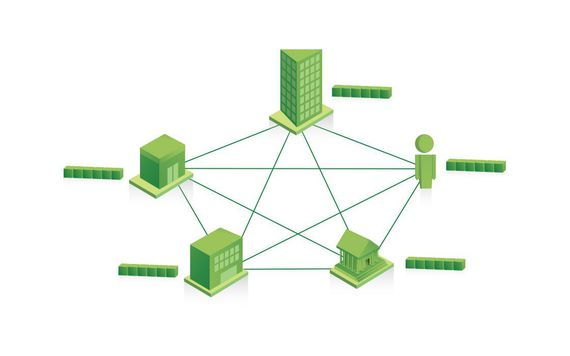
\includegraphics[scale=0.25]{proposed.jpg}
		\captionof{figure}{Topologie sistem descentralizat}
	\end{center}
	\begin{itemize}%[<+- | alert@+>]
	
  			\item {\small Fiecare institutie implicata detine o copie a inregistrarilor din retea}
  			\item {\small Partajarea datelor simplificata}
  			\item {\small Imutabilitatea datelor, modificarile asupra inregistrarilor fiind observate de toti participantii}	
  			\item {\small Eficienta crescuta in detectarea fraudelor}
  	\end{itemize}
  \end{frame}
  \section{Tehnologii folosite}
  \begin{frame}{Hyperledger Fabric}
  	
\includegraphics[scale=0.25]{fabric.png}

  	\begin{itemize}
  		\item Framework pentru realizarea unei retele blockchain
  		\item Arhitectura descentralizata
  		\item Suport pentru smart contracts
  		\item Open-source
  	\end{itemize}
  \end{frame}
  \begin{frame}{Hyperledger Composer}
  	
\includegraphics[scale=0.25]{comp.png}
  	\begin{itemize}
  		\item Ofera unelte pentru simplificarea procesului de dezvoltare al aplicatiilor pe blockchain
  		\item Suport pentru implementarea cazurilor de utilizare 
  		\item Simplifica integrarea cu sisteme deja existente
  		\item Suport pentru definirea punctelor de acces in retea pentru utilizatorii finali
  	\end{itemize}
  \end{frame}   
  \section{Analiza si design}
  \begin{frame}{Arhitectura sistem}
  	\begin{center}
  		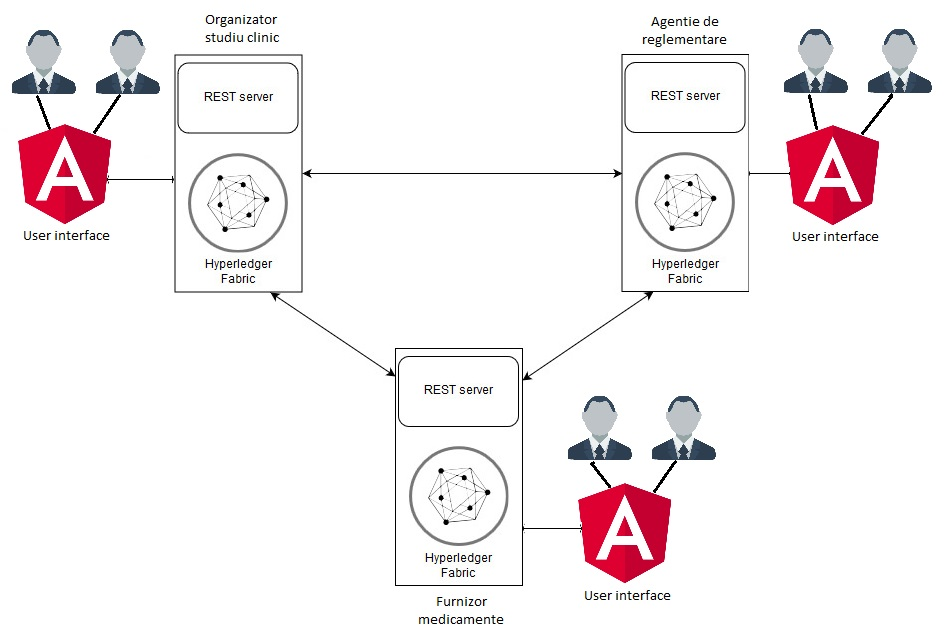
\includegraphics[scale=0.42]{arh.jpg}
  	\end{center}
  \end{frame}
  \begin{frame}{Arhitectura nod sistem}
  	\begin{center}
  		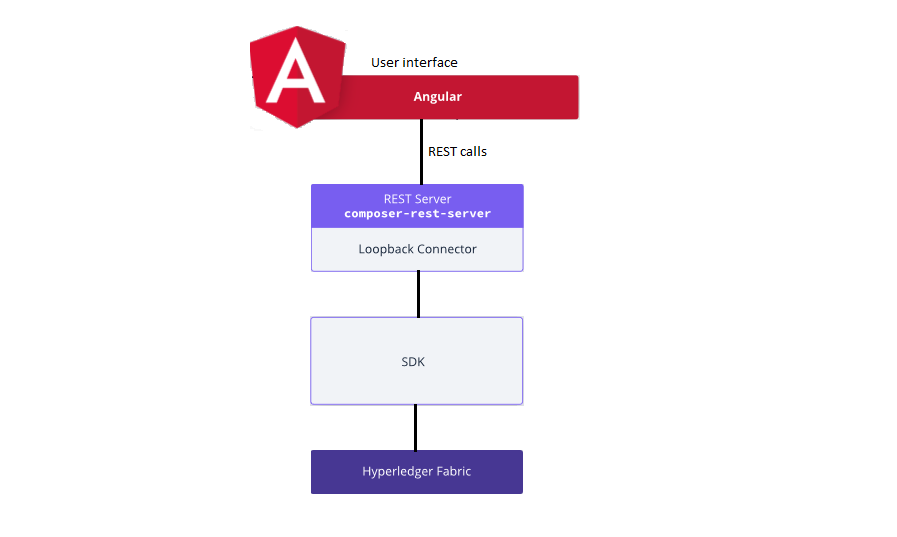
\includegraphics[scale=0.42]{hyp_fab.PNG}
  	\end{center}
  \end{frame}
  \begin{frame}{Definirea retelei blockchain - Hyperledger Composer}
  		\begin{center}
  		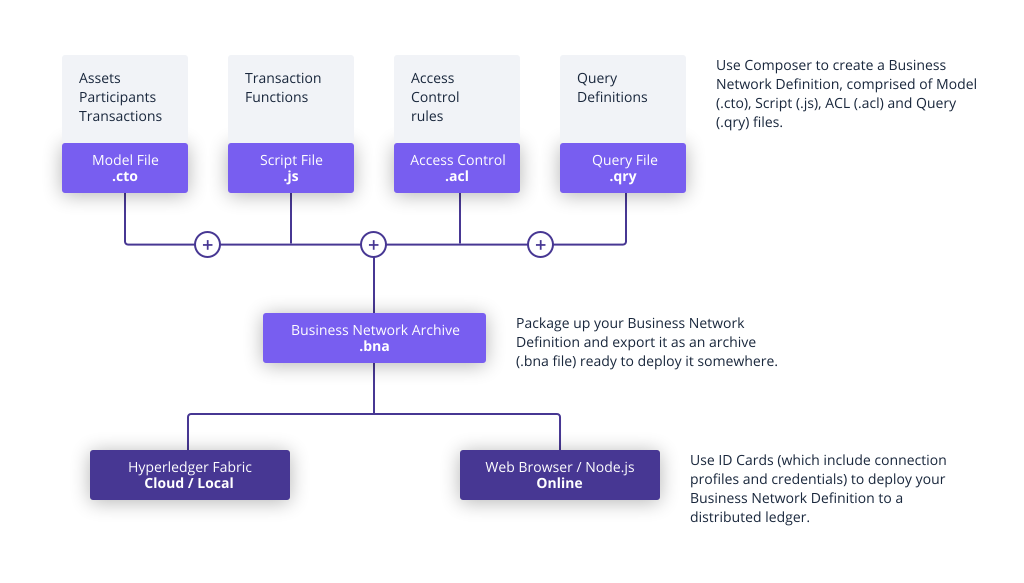
\includegraphics[scale=0.4]{Composer-Diagram.png}
  		\end{center}
  \end{frame}   
  \begin{frame}{Concepte} 	
 	\begin{itemize}
 		\item \textbf{Asset-uri} - obiectele tranzactionate in retea, identificate printr-un ID unic(ex. studiul clinic poate fi definit ca un asset).
 		\item \textbf{Participanti} - membrii retelei blockchain. 
 		\item \textbf{Tranzactii} - definesc modul de interactiune dintre asset-uri si participanti
 		\item \textbf{Reguli de acces} - specifica resursele la care are acces un anumit participant
 		\item \textbf{Intergoari} - folosite pentru obtinerea de date din reteaua blockchain 
 	\end{itemize}
  \end{frame}
  \begin{frame}[fragile]{Exemple - concepte}
  	\begin{Verbatim}[fontsize=\small]
/** Clinic trial represented as an asset*/
asset Trial identified by idTrial{
    o String idTrial
    o ProtocolEntry[] protocolEntries optional
    o TrialDetails details optional
    o TrialStatus status optional
    -->Patient[] participants optional
    -->Researcher organiser
}

/** Transaction for registering a new clinic trial*/
transaction RegisterTrialTransaction  {
    o String idTrial
    o TrialDetails details optional
    -->Researcher organiser
}
  	\end{Verbatim}
  \end{frame}
  \begin{frame}[fragile]{Exemplu - tranzactie}
  	\begin{Verbatim}[fontsize=\tiny]
/**
 * Register a new trial, add the required relationships and set the trial status
 * @param {ro.utcluj.clinictrial.RegisterTrialTransaction} trialRequest - Transaction
 * to be processed
 * @transaction
 */
function registerTrialTransaction(trialRequest){
    var factory = getFactory();
    //namespace definitions
    var namespace_trial = 'ro.utcluj.clinictrial.trial'
    var namespace_person = 'ro.utcluj.clinictrial.base'

    var trial = factory.newResource(namespace_trial, 'Trial', trialRequest.idTrial);
    trial.details = trialRequest.details;
    trial.status = 'REGISTERED';

    //add the relationship to the Researcher that created the clinic trial
    trial.organiser = factory.newRelationship(namespace_person, 'Researcher',
                            trialRequest.organiser.getIdentifier());

    // save the asset
    return getAssetRegistry(trial.getFullyQualifiedType())
            .then(function (assetRegistry) {
                      return assetRegistry.add(trial);
  })
} 	
  	\end{Verbatim}
  \end{frame}
  \begin{frame}[fragile]{Exemplu - Reguli de acces}
  	\begin{Verbatim}[fontsize=\tiny]
/**
 * Access control rules for clinic trial
 */
rule Default {
  description: "Allow all participants access to all resources"
  participant: "ANY"
  operation: ALL
  resource: "ro.utcluj.clinictrial.*"
  action: ALLOW
}

rule SystemACL {
  description:  "System ACL to permit all access"
  participant: "ANY"
  operation: ALL
  resource: "org.hyperledger.composer.system.**"
  action: ALLOW
}
	\end{Verbatim}
  \end{frame}
  \begin{frame}[standout]
  Intrebari?
  \end{frame}
  
  \begin{frame}[allowframebreaks]{References}

  \bibliography{demo}
  \bibliographystyle{abbrv}

\end{frame}
\end{document}